%% Copernicus Publications Manuscript Preparation Template for LaTeX Submissions
%% ---------------------------------
%% This template should be used for copernicus.cls
%% The class file and some style files are bundled in the Copernicus Latex Package, which can be downloaded from the different journal webpages.
%% For further assistance please contact Copernicus Publications at: production@copernicus.org
%% https://publications.copernicus.org/for_authors/manuscript_preparation.html

%% copernicus_rticles_template (flag for rticles template detection - do not remove!)

%% Please use the following documentclass and journal abbreviations for discussion papers and final revised papers.

%% 2-column papers and discussion papers
\documentclass[soil, manuscript]{copernicus}



%% Journal abbreviations (please use the same for preprints and final revised papers)

% Advances in Geosciences (adgeo)
% Advances in Radio Science (ars)
% Advances in Science and Research (asr)
% Advances in Statistical Climatology, Meteorology and Oceanography (ascmo)
% Aerosol Research (ar)
% Annales Geophysicae (angeo)
% Archives Animal Breeding (aab)
% Atmospheric Chemistry and Physics (acp)
% Atmospheric Measurement Techniques (amt)
% Biogeosciences (bg)
% Climate of the Past (cp)
% DEUQUA Special Publications (deuquasp)
% Earth Surface Dynamics (esurf)
% Earth System Dynamics (esd)
% Earth System Science Data (essd)
% E&G Quaternary Science Journal (egqsj)
% EGUsphere (egusphere) | This is only for EGUsphere preprints submitted without relation to an EGU journal.
% European Journal of Mineralogy (ejm)
% Fossil Record (fr)
% Geochronology (gchron)
% Geographica Helvetica (gh)
% Geoscience Communication (gc)
% Geoscientific Instrumentation, Methods and Data Systems (gi)
% Geoscientific Model Development (gmd)
% History of Geo- and Space Sciences (hgss)
% Hydrology and Earth System Sciences (hess)
% Journal of Bone and Joint Infection (jbji)
% Journal of Micropalaeontology (jm)
% Journal of Sensors and Sensor Systems (jsss)
% Magnetic Resonance (mr)
% Mechanical Sciences (ms)
% Natural Hazards and Earth System Sciences (nhess)
% Nonlinear Processes in Geophysics (npg)
% Ocean Science (os)
% Polarforschung - Journal of the German Society for Polar Research (polf)
% Primate Biology (pb)
% Proceedings of the International Association of Hydrological Sciences (piahs)
% Safety of Nuclear Waste Disposal (sand)
% Scientific Drilling (sd)
% SOIL (soil)
% Solid Earth (se)
% State of the Planet (sp)
% The Cryosphere (tc)
% Weather and Climate Dynamics (wcd)
% Web Ecology (we)
% Wind Energy Science (wes)

% Pandoc citation processing

% The "Technical instructions for LaTex" by Copernicus require _not_ to insert any additional packages.
% % % From pandoc table feature
% \usepackage{longtable,booktabs,array}
% % \usepackage{calc} % for calculating minipage widths
% % Correct order of tables after \paragraph or \subparagraph
% \usepackage{etoolbox}
% \makeatletter
% \patchcmd\longtable{\par}{\if@noskipsec\mbox{}\fi\par}{}{}
% \makeatother
% % Allow footnotes in longtable head/foot
% \IfFileExists{footnotehyper.sty}{\usepackage{footnotehyper}}{\usepackage{footnote}}
% \makesavenoteenv{longtable}
% 
% tightlist command for lists without linebreak
\providecommand{\tightlist}{%
  \setlength{\itemsep}{0pt}\setlength{\parskip}{0pt}}


%
%% \usepackage commands included in the copernicus.cls:
%\usepackage[german, english]{babel}
%\usepackage{tabularx}
%\usepackage{cancel}
%\usepackage{multirow}
%\usepackage{supertabular}
%\usepackage{algorithmic}
%\usepackage{algorithm}
%\usepackage{amsthm}
%\usepackage{float}
%\usepackage{subfig}
%\usepackage{rotating}

\begin{document}


\title{Wall-to-wall mapping of peat depth from Lidar terrain and airborne radiometrics in Norwegian landscapes}


\Author[1][julien.vollering@hvl.no]{Julien}{Vollering}
\Author[2]{Naomi}{Gatis}
\Author[1]{Mette}{Kusk Gillespie}
\Author[1]{Karl-Kristian}{Muggerud}
\Author[1]{Sigurd Daniel}{Nerhus}
\Author[1]{Knut}{Rydgren}
\Author[1]{Mikko}{Sparf}


\affil[1]{Department of Civil Engineering and Environmental Sciences, Western Norway University of Applied Sciences, Norway}
\affil[2]{Department of Geography, University of Exeter, United Kingdom}

\runningtitle{Peat depth from terrain and radiometrics}

\runningauthor{Vollering et al.}


\correspondence{Julien\ Vollering\ (julien.vollering@hvl.no)}



\received{}
\pubdiscuss{} %% only important for two-stage journals
\revised{}
\accepted{}
\published{}

%% These dates will be inserted by Copernicus Publications during the typesetting process.


\firstpage{1}

\maketitle


\begin{abstract}
The abstract goes here.
It can also be on \emph{multiple lines}.
\end{abstract}




\section{Introduction}

Peat soils are a terrestrial carbon stock of global importance.
They store about 30 \% of global soil carbon despite covering only 2-3 \% of Earth's land \citep{xuPEATMAPRefiningEstimates2018, friedlingsteinGlobalCarbonBudget2020, unepGlobalPeatlandsAssessment2022}.
In other words, they are extremely carbon dense -- denser than any other ecosystem per square meter \citep{temminkRecoveringWetlandBiogeomorphic2022}.
This makes peatlands crucial to climate change mitigation.
Intact peatlands sequester carbon and produce a negative temperature forcing, overall \citep{joostenRolePeatlandsClimate2016}.
When disturbed, often by conversion to another land use, they can produce large greenhouse gas emissions \citep{maGloballyRobustRelationship2022}.

One of the keys to the areal density of peatland carbon stocks lies in the third dimension: their depth.
Peat soils range from zero to over ten meters deep, so deep peats comprise a large volume.
Their depth results from the accumulation of organic matter over thousands of years \citep{loiselDatabaseSynthesisNorthern2014, joostenRolePeatlandsClimate2016}.
In the anoxic and acidic conditions created by a high water table, plant material decay is slightly outweighed by new growth, and the surplus carbon is laid down as peat.
There it remains sequestered as long as the water table stays high and prevents oxidation.

Peatlands are unevenly distributed globally, and in regions with high cover they are frequently converted to human land use \citep{unepGlobalPeatlandsAssessment2022}.
They are attractive for agriculture and forestry because they are flat, treeless, and have developed soils.
However, other land uses also displace peatlands.
In Norway, where 9\% of the land area is peatland \citep{brynLandCoverNorway2018}, construction and development have become important drivers of loss, after lawmakers restricted conversion to forest and farmland in recent decades.

The spatial distribution of peat depth is often overlooked in land use planning and carbon accounting because peat depth is not mapped with sufficient coverage, resolution, or accuracy.
Maps are crucial because they link high-level targets to specific management decisions, unlike spatially aggregated estimates \citep{oecdOECDEnvironmentalPerformance2022}.
For example, Norwegian regulations restrict conversion to farmland more strictly where peat depth exceeds \unit{1\,m}, and the distribution of peat depth on a farmer's property determines whether he is allowed to convert peatland (Forskrift om nydyrking, 1997, § 5a).
Maps also make it possible to quantify the effect of specific management decisions and thereby understand how local outcomes contribute to regional and national outcomes \citep{oecdOECDEnvironmentalPerformance2022}.

Measuring peat depth on the ground is straightforward, and a field survey can map a small area at low cost.
However, surveying large areas is impractical when depth varies over short distances -- as in most peatlands.
A complementary approach from soil science is digital soil mapping (DSM).
DSM scales up field measurements from a set of locations to a wider area, by relating the measured values to other variables mapped over the area of interest.
This approach has grown important with the availability of remotely sensed data and the advancement of methods for identifying pattern, especially through machine learning \citep{minasnyDigitalMappingPeatlands2019, wadouxMachineLearningDigital2020}.

The crux for DSM of peat depth are the relationships between peat depth and the other, mapped variables.
For DSM to work, these relationships must be strong and consistent over the area of interest.
They can be purely correlative rather than causal, but mechanistic relationships are stronger and more consistent.
The \emph{scorpan} framework for DSM suggests seven predictor classes to explore: other soil properties, climate, organisms, relief (topography), parent material, age, and spatial position \citep{mcbratneyDigitalSoilMapping2003}.

The most practical and widespread \emph{scorpan} factors for peat depth are relief and spatial position.
Spatial position is unique because it is always known (with varying accuracy).
However, the short range of spatial autocorrelation in peat depth limits its mapping value \citep{henglGenericFrameworkSpatial2004}.
Relief, or topography, is widely and accurately mapped in digital terrain models.
For example, most of mainland Norway has at least one elevation measurement per square meter from airborne LiDAR surveys.
Moreover, mechanisms of peat formation are linked to topography.
For example, a steep slope is unlikely to have a high water table, thereby limiting accumulation.

Studies have consistently shown relationships between peat depth and topography, although the specific patterns vary.
One of the most robust relationships is a negative correlation between depth and terrain slope \citep[e.g.][]{holdenEstimatingCarbonStock2011, parryMethodModellingPeat2012, gatisMappingUplandPeat2019}.
Peat depth also changes with elevation in many contexts, but with inconsistent directionality \citep[e.g.][]{holdenEstimatingCarbonStock2011, parryMethodModellingPeat2012, rudiyantoDigitalMappingCosteffective2016, rudiyantoOpenDigitalMapping2018, kogantiMappingPeatDepth2023, liFactorsControllingPeat2024}.
Also more complex derivations of topography, such as the Topographic Wetness Index (TWI) and the Multi-Resolution Valley Bottom Flatness (MRVBF) index, have shown associations with peat depth in some studies \citep[e.g.][]{rudiyantoOpenDigitalMapping2018, kogantiMappingPeatDepth2023, liFactorsControllingPeat2024}.
Some of the variation between studies in quantifying these relationships is undoubtedly attributable to issues of spatial scale -- both the scaling of the topographic variables and the resolution of the peat depth analysis.

Another set of variables related to peat depth are measurements of natural radioactivity from the ground surface.
Gamma-ray spectrometry can survey the activity (decay counts per second) from radioactive isotopes in the earth's crust: potassium-40, uranium-238, and thorium-232 \citep{reinhardtGammaraySpectrometryVersatile2019}.
These exist in bedrock (and mineral soils) and a peat overburden attenuates the radiation intensity at the surface.
The degree of attenuation relates to properties of the overburden, especially composition and depth.
Deep soil with high water content attenuates most \citep{beamishGammaRayAttenuation2013, reinhardtGammaraySpectrometryVersatile2019}.
Thus, gamma-ray radiometrics integrate the \emph{scorpan} factors soil, parent material, and age.

Although theory suggests that one meter of peat may fully attenuate radiometric signal \citep{beamishGammaRayAttenuation2013, reinhardtGammaraySpectrometryVersatile2019}, empirical investigations show that the association between peat depth and radioactivity can extend beyond the first meter \citep{gatisMappingUplandPeat2019, kogantiMappingPeatDepth2023}.
Radiometric data are increasingly available over large areas, presenting a big opportunity insofar as they are predictive.
Airborne surveys are used for various applications, and some countries have high spatial coverage of such data \citep{minasnyDigitalMappingPeatlands2019, baranwalAirborneGeophysicalSurveys2020}.

The effectiveness of DSM depends not only on the methods and data, but also on the characteristics of the mapping area.
Norway may be instructive in this respect because its peatlands vary widely across climates and topographies. There are many mire massif types, with different hydrology, formation, and development -- from topogeneous or soligeneous fens to blanket or raised bogs \citep{lyngstadBeskrivelserAvTorvmassivenheter2023}.
These types have fundamentally different geomorphology, suggesting that peat depth relationships with terrain or radiometric variables will vary by landscape.

The little we know about the depths of Norwegian peatlands comes from surveys meant to identify arable land.
After scattered surveys in the early 20th century, a comprehensive round of surveying was completed 1964-2001 as part of a wider land cover mapping in Norway \citep{bjordalMarkslagsklassifikasjonOkonomiskKartverk2007}.
Because of its agricultural and silvicultural focus, it covered only productive areas below the tree line, and peat depth was measured only in places judged to be potentially arable or afforestable \citep{ahlstromAR5Klassifikasjonssystem2019}.
Field surveyors carried a one-meter probe, so they measured peat depth as shallow (\textless{} 1 m), or deep (\textgreater{} 1 m).
These classes were assigned to whole mire polygons, so spatial resolution is on the order of hectares.

Soil science needs more studies of relationships between peat depth and topographic or radiometric data to determine how predictive they are, which variables are most predictive, and how consistent their associations.
The push for nature-based climate solutions motivates for broad mapping of peat depth, to identify rich peatland carbon stocks and avoid their conversion.
Although small areas can be mapped accurately on the ground, having landscape-scale maps \emph{before} detailed investigation increases the option space for spatial planning and land management.
For example, the Norwegian Public Roads Administration routinely measures peat depth during geotechnical work, but by that time, the route of the road is already set.
With a digital peat depth map, planners could better compare routes and climate mitigation measures would have more leverage.

We assess how well remotely sensed topographic and radiometric data can predict peat depth at the landscape scale, with a view towards revising regional and national maps in Norway.
Specifically, we: (1) quantify the accuracy of predictions from topographic and radiometric variables, (2) identify key predictive variables, and (3) compare these relationships across two different Norwegian landscapes.
To our knowledge, this is the first study to predict peat depth from airborne radiometric data using machine learning algorithms.
Where airborne radiometric data have been used to predict peat depth, it has been through modeling techniques less suited for prediction and spatial extrapolation \citep[e.g.,][]{keaneySpatialStatisticsEstimate2013, gatisMappingUplandPeat2019, siemonAirborneElectromagneticRadiometric2020}.
Where machine learning algorithms have been used on airborne radiometric data, it has been to predict peat extent rather than depth \citep[e.g.,][]{olearyDigitalSoilMapping2022}.

\section{Materials and methods}

\subsection{Sites}

We assessed how well we could predict peat depth at two sites with conspicuously different physical geography: Skrimfjella in eastern Norway and Ørskogfjellet in western Norway (Fig. \ref{fig:sites}c).
These sites were chosen because they were covered by radiometric data from airborne surveys, relatively little built-up area, and road access.

\begin{figure}
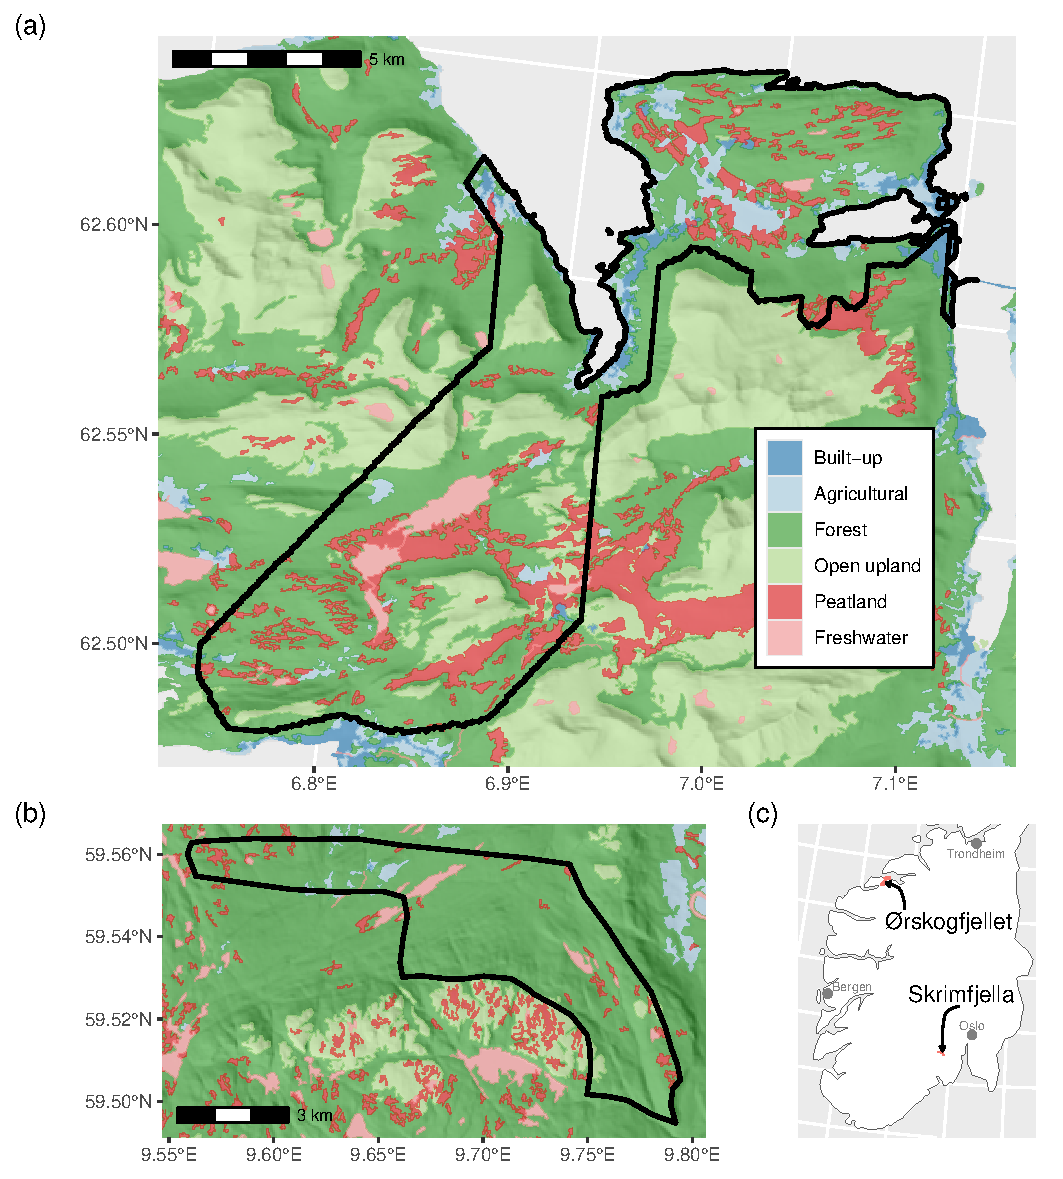
\includegraphics[height=0.9\textheight]{figures/sites-patchwork} \caption{Study areas at Ørskogfjellet (a) and Skrimfjella (b) within southern Norway (c). Land cover shown here is from the AR50 national land resource database and has simplified geometry with respect to the AR5 database used in the study.}\label{fig:sites}
\end{figure}

At Skrimfjella we delineated a study area of \unit{34\,km^{2}} based on radiometric coverage and accessibility (Fig. \ref{fig:sites}b).
The study area has a diverse bedrock, with 32 \% alkali feltspat granite, 26 \% mergelstein, 10 \% granite, and eight other types with \textgreater{} 1 \% coverage (NGU, 1:250 000 dataset).
The landscape within our delineation is classified as \emph{inland hills and mountains} \citep{simensenDiversityDistributionLandscape2021}.
It is almost without human infrastructure, dominated by forest, and borders on a large nature reserve.
The study area has a mean elevation of \unit{438\,m} above sea level (range 223--711, IQR 351--509), and its mean slope at \unit{10\,m} resolution is 10.8° (IQR 4.6--15.1°).
In Norway's AR5 national land capability dataset \citep{ahlstromAR5Klassifikasjonssystem2019}, \unit{1.5\,km^{2}} (4.5 \%) of the study area is classified as mire -- defined as areas with mire vegetation and at least \unit{30\,cm} of peat depth.

At Ørskogfjellet we defined a study area of \unit{124\,km^{2}} which basically followed the footprint of the radiometric survey (Fig. \ref{fig:sites}a).
According to the Geological Survey of Norway, bedrock in the area is 84 \% granitic gneiss, 11 \% granite, and 5 \% aluminium silicate gneiss (NGU, 1:250 000 dataset).
This study area comprises a wide range of major landscape types: \emph{coastal plains}, \emph{coastal fjord}, \emph{inland valleys}, as well as \emph{inland hills and mountains} \citep{simensenDiversityDistributionLandscape2021}.
It is mostly forested, but also contains considerable farmland and open upland, and has several large lakes.
Its mean elevation is \unit{211\,m} above sea level (range 0--807, IQR 73--310), and its mean slope at \unit{10\,m} resolution is 13.0° (IQR 4.7--18.3°).
The AR5 dataset counts \unit{15.3\,km^{2}} (12.4 \%) of the study area as mire.

\subsection{Peat depth measurements}

At both study sites, our measurements of peat depth were made for the purpose of training a Random Forest (RF) model of peat depth, and we designed our sampling with this in mind \citep{brusSamplingDigitalSoil2019}.
Broadly, we aimed for a sample that was representative of the predictor space defined by the most important predictors of peat depth \citep{wadouxSamplingDesignOptimization2019, maComparisonConditionedLatin2020}.
A sample that preserves the properties of the multivariate distribution of predictor and outcome variables is most likely to maintain any complex, non-linear relationships that exist in the population while avoiding spurious ones \citep{brusSamplingDigitalSoil2019}.
We chose for our sampling and modelling a spatial resolution of \unit{10\,m}.
We considered this a reasonable compromise between digital terrain model (DTM) resolution (\unit{1\,m}) and small mires on the one hand, and airborne radiometric resolution (\unit{50\,m}) on the other.
The point measurements of peat depth described below were ultimately aggregated to \unit{10\,m} resolution by taking the mean of point values within each cell, inversely weighted by their distances to the cell center.

\subsubsection{Skrimfjella}

We measured peat depth in selected locations (\unit{10\,m} raster cells) at Skrimfjella.
The locations were chosen only from areas delineated as mire in the AR5 national land capability dataset.
Within this mire area, we stratified our sample across values of elevation, slope, and potassium ground concentration \citep[from processed airborne gamma ray spectrometry,][]{baranwalHelicopterborneMagneticElectromagnetic2013}.
Specifically, we used the \emph{eSample} function in the \emph{iSDM} R package (v.1.0) to chose an environmentally systematic sample.
This function defines the environmental space as a two-dimensional convex hull around the ordinated data, then creates a regular grid across that space, and lastly finds for each grid cell the datum that is nearest \citep{hattabUnifiedFrameworkModel2017}.
Elevation was extracted from the \unit{10\,m} national DTM, slope calculated in degrees, and potassium ground concentration downscaled with bilinear resampling.
We set a target sample size of 100, excluded the top and bottom percentile from the convex hull, and with these parameters \emph{eSample} returned 105 raster cells.

In addition to the peat depth locations, we had another arm of our sampling design for measuring peatland occurrence, as a binary variable.
We wanted to measure peatland occurrence outside of mapped mire areas because the AR5 dataset is known to underestimate peatland coverage \citep[especially in forests,][]{brynLandCoverNorway2018}, and because airborne radiometrics may help identify unmapped peatland \citep{gatisMappingUplandPeat2019, olearyDigitalSoilMapping2022}.
The occurrence locations were sampled from the part of the study area that (1) was mapped as something other than mire in the AR5 database and (2) had a slope \textless{} 20°.
We performed environmentally systematic sampling of this population with the same procedure as for the depth locations, and \emph{eSample} returned 106 raster cells.

Field work at Skrimfjella was conducted in August 2020.
We navigated to the centers of the raster cells in the depth and occurrence samples by handheld GPS, checking that positional error was below \unit{3\,m}.
For each depth sample location, we measured peat depth three times (at the vertices of a triangle with \unit{2\,m} sides) to get a more representative value for the \unit{10\,m} raster cell, and to dampen the effect of outlying measurements \citep{parryEvaluatingApproachesEstimating2014}.
We used a metal probe pushed downward until resistance indicated the base of the peat column.
Probe locations were adjusted up to \unit{20\,cm} if the base of the peat column seemed to be blocked by an obvious artifact.
A single probe measurement was right-censored because the peat column was deeper than the probe.
For each occurrence sample location, we recorded the presence or absence of peatland -- primarily by digging and examining the top \unit{20\,cm} of soil (where this was possible).
We judged whether the soil was a peat soil based on its density, texture, and color.
Occasionally, when the soil itself was difficult to judge, we made our determination also based on the presence or absence of mire vegetation.
Although peat soil is strictly defined by organic content (which we did not analyse), we believe our protocol produced reasonable determinations of presence or absence that would generally satisfy most of the varying definitions of peatland \citep{minasnyMappingMonitoringPeatland2023}.

Besides the depth and occurrence measurements described above, we also measured peat depth in three subjectively-chosen, individual mires, using ground-penetrating radar (GPR).
We used the Malå ProEx GPR system (Guideline Geo AB, Sweden) with its \unit{500\,MHz} shielded antenna mounted in a plastic sledge, and its control unit connected to a GNSS receiver.
At each of the three mires we recorded GPR traces along walking transects that covered the extent of the mire, mostly in traversing, zigzag patterns with between \unit{5\,m} and \unit{20\,m} spacing at their vertices.
Along the GPR transects we also probed peat depth at marked trace locations, to be able to calibrate the GPR wave speed velocity.
We processed the GPR data with Reflex2DQuick software (v.3.0, Sandmeier Scientific Software, Germany), applying a time-zero correction, a dewow filter, and a gain filter based on observed energy decay.
Then we picked strong reflectors in the radargrams that we interpreted as the base of the peat column.
We used picks at marked trace locations to calibrate wave speed velocity; we pooled calibration points across the three mires and fitted a linear regression of depth on one-way travel time with the intercept fixed at zero.
In total we had 46 calibration points along \unit{3.5\,km} of GPR transects.
Finally, we used the calculated wave velocity (\unit{0.0387\,m\,ns^{-1}}, \(R^2 = 0.874\)) to convert the travel times of all picks to calibrated peat depths.

\subsubsection{Ørskogfjellet}

At Ørskogfjellet we also measured peat depth in a sample of \unit{10\,m} raster cells, selected from the part of the study area classified in the AR5 dataset as mire.
Before selecting locations, we determined a minimal sample size that would adequately capture the terrain and radiometric properties of the entire mire area.
Specifically, we aimed to identify the size at which adding locations produced diminishing decreases in divergence between sample and population distributions -- i.e.~the elbow point in a curve of similarity between sample and population \citep{maloneMethodsImproveUtility2019}.
This approach has been found to identify sample sizes that correspond with diminishing returns in predictive model performance on external evaluation data \citep{sauretteDivergenceMetricsDetermining2023}.
We defined a sequence of sample sizes (50--500) and for ten replicate samples at each size \citep[drawn by conditioned latin hypercube sampling,][]{minasnyConditionedLatinHypercube2006, roudierClhsPackageConditioned2011}, we calculated the mean Kullback-Leibler divergence between sample and population distributions \citep{maloneMethodsImproveUtility2019, sauretteDivergenceMetricsDetermining2023}.
The predictors in the divergence calculation were terrain slope and four radiometrics: potassium, thorium, uranium, and total count.
Next, we fitted a asymptotic regression of mean divergence on sample size, and identified the sample size at which the curve reached 95 \% of the fitted asymptote.
Through this procedure we found that we could adequately capture the population distribution with a sample of 160 locations.

To choose 160 locations, we performed feature space coverage sampling.
This approach has been found to produce higher accuracy in RFs than conditioned latin hypercube sampling \citep{wadouxSamplingDesignOptimization2019, maComparisonConditionedLatin2020}.
Feature space coverage sampling aims to disperse samples as uniformly as possible in multidimensional predictor space, and is implemented by choosing locations that are closest to cluster centers in a k-means clustering of the standardized predictor space \citep{brusSamplingDigitalSoil2019}.
Feature space coverage sampling works best when all dimensions are important predictors of the outcome \citep{wadouxSamplingDesignOptimization2019}, and we used the same five predictors that we used to choose sample size: terrain slope and four radiometrics.
The radiometric predictors were downscaled to \unit{10\,m} resolution with cubic B-spline resampling in QGIS \citep[v.3,][]{QGISsoftware}.
We adjusted the feature space coverage sampling to ensure that locations were accessible within time constraints, and assessed how this changed our sample from an ideal feature space coverage sample.
Adjusting for accessibility is justified because the smaller sample size that would result if accessibility were ignored can degrade model accuracy as much or more as deviations from ideal sampling designs \citep{wadouxSamplingDesignOptimization2019, maComparisonConditionedLatin2020}.
To adjust, we first restricted the sampling population to mire areas that were within an arbitrary cost distance of publicly-accessible roads.
Cost distance was calculated using GRASS's \emph{r.walk} function, with friction costs defined by AR5 land classes \citep{GRASSv8-2}.
After creating a feature space coverage sample with this restriction, we also inspected a map of the sample and substituted 16 inaccessible locations with accessible locations from the same or a nearby cluster.
Our two accessibility adjustments increased the distance in standardized predictor space between sample locations and cluster centers by 78 \% (with respect to the ideal sample), but distance in our sample was still only 46 \% of the mean distance to cluster centers -- i.e., accessibility did not force locations far from cluster centers relative to the size of the clusters.

Field work at Ørskogfjellet was conducted in August 2023.
We navigated to the centers of the raster cells in the sample using real time kinematic differential GNSS (Topcon Positioning Systems, USA), to ensure sub-meter positional accuracy.
At each location we measured peat depth three times by manual probing, with probe locations spaced approximately \unit{2.5\,m} apart.
For a tiny fraction of these measurements (5 total), it was not possible to reach the base of the peat column, and a right-censored depth was recorded.
In areas with dense sampling locations, we also measured peat depth with GPR along snaking transects passing through the centers of the sampling cells (seven transects, \unit{6.2\,km} total length).
We used the same GPR system as at Skrimfjella, but with a \unit{100\,MHz} Malå rough terrain antenna (Guideline Geo AB, Sweden) at some transects.
To navigate the GPR transects, we placed flags at the cell centers of the sample locations, and used a handheld GNSS receiver to guide the GPR operator.
At sampling locations crossed by a GPR transect, we arranged the manual probe positions along the transect (for better calibration of the GPR wave speed velocity), while other locations were probed in a triangular pattern around the cell center like at Skrimfjella.

We processed the GPR data with Reflexw software (v.8.5, Sandmeier Scientific Software, Germany), applying a dewow filter, time-zero correction, bandpass filter, gain filter, and a dynamic correction that accounts for the non-vertical wave path between offset transmitter and receiver antennae.
The last correction is important for the rough terrain antenna, which has an antenna separation (\unit{2.2\,m}) -- comparable to typical peat depths.
As with the data from Skrimfjella, we picked the base of the peat column from strong reflectors in the radargram, and calibrated wave velocity with manual probe measurements in a linear regression.
The points in the regression were created by joining to each probe measurement the travel time of the nearest pick, but only if these were within \unit{2\,m} of each other.
In total we had 78 calibration points along \unit{7.8\,km} of interpretable GPR traces (transect length exceeded because of extra GPR data).
Finally, we used the calculated wave velocity (\unit{0.0427\,m\,ns^{-1}}, \(R^2 = 0.946\)) to convert the travel times of all picks to calibrated peat depths.

We also used two sets of existing depth measurements from Ørskogfjellet.
The first set was provided by the Norwegian Public Roads Administration, who commissioned GPR surveys of particular peatland areas in 2020 and 2021.
The surveys were conducted with a dual channel system (\unit{70\,MHz} and \unit{300\,MHz}; ImpulseRadar AB, Sweden), connected to GNSS with CPOS correction.
We used interpreted and calibrated traces from these surveys, and discarded some data where multiple depths were interpreted for the same locations.
This summed to \unit{7.4\,km} of interpreted traces.
The second set of existing depth data we extracted from a paper map made by the Norwegian Soil and Mire Company in 1984.
This map presents 44 borehole depths (in decimeters) across a \unit{9\,ha} peatland area.
We georeferenced the map and digitized the borehole locations and depths.

\subsection{Peat depth predictors}

We created the same suite of peat depth predictors for both sites (25 continuous and 1 categorical; Table \ref{tab:preds}).
All continuous predictors were derived either from an airborne radiometric survey or from a DTM.
From the radiometric surveys we simply used the four variables produced by the surveyors (Geological Survey of Norway): ground concentration of Potassium, Thorium, Uranium, as well as total count.
From the DTMs we calculated several land surface parameters, ranging from simple terrain indices to more complex geomorphometric and hydrological variables \citep{maxwellLandsurfaceParametersSpatial2022}.
The categorical predictor was peat depth class, from a national map dataset.
Complete descriptions of predictors follow below.

\begin{table}

\caption{\label{tab:preds}Candidate predictors of peat depth.}
\centering
\begin{tabular}[t]{ll}
\hline
Name & Description\\
\hline
radK & Potassium ground concentration\\
radTh & Thorium ground concentration\\
radU & Uranium ground concentration\\
radTC & Total count of gamma radiation\\
elevation & Mean elevation\\
slope1m & Mean of 1 m slope\\
TPI1m & Mean of 1 m topographic position index\\
TRI1m & Mean of 1 m terrain ruggedness index\\
roughness1m & Mean of 1 m roughness\\
slope10m & 10 m slope\\
TPI10m & 10 m topographic position index\\
TRI10m & 10 m terrain ruggedness index\\
roughness10m & 10 m roughness\\
MRVBF & Multi-resolution valley bottom flatness\\
TWI5m & Mean of 5 m topographic wetness index\\
TWI10m & 10 m topographic wetness index\\
TWI20m & Bilinear interpolation of 20 m topographic wetness index\\
TWI50m & Bilinear interpolation of 50 m topographic wetness index\\
DTW2500 & Depth-to-water index, flow initiation area of 0.25 ha\\
DTW5000 & Depth-to-water index, flow initiation area of 0.5 ha\\
DTW10000 & Depth-to-water index, flow initiation area of 1 ha\\
DTW20000 & Depth-to-water index, flow initiation area of 2 ha\\
DTW40000 & Depth-to-water index, flow initiation area of 4 ha\\
DTW80000 & Depth-to-water index, flow initiation area of 8 ha\\
DTW160000 & Depth-to-water index, flow initiation area of 16 ha\\
DMK & DMK peat depth class, categorical with 3 levels\\
\hline
\end{tabular}
\end{table}

\subsubsection{Radiometric}

The radiometric survey covering Skrimfjella was conducted in 2008--2011.
The survey was flown at an average altitude of \unit{75\,m} and average speed of \unit{108\,km\,h^{-1}}, with flight lines spaced \unit{200\,m} apart.
Spectrometer count rates were calibrated annually to known concentrations of Potassium, Thorium, and Uranium in mobile pads.
The Geological Survey of Norway processed data from the spectrometer following standard procedures outlined by the International Atomic Energy Association, and the processing included: correction for aircraft and cosmic background radiation, correction for radon in the air, window stripping of the gamma ray spectrum, correction for flying height, conversion of count rates to ground concentrations, and finally gridding to \unit{50\,m} resolution with micro-leveling.
Further details about the survey and data processing are provided in Baranwal et al. \citeyearpar{baranwalHelicopterborneMagneticElectromagnetic2013}.
We downscaled the processed data to \unit{10\,m} resolution by cubic spline resampling, using the \emph{terra} package in R.

A very similar radiometric survey covering Ørskogfjellet was conducted in December 2014 and January 2015.
This survey was flown at an average altitude of \unit{80\,m} and average speed of \unit{88\,km\,h^{-1}}, with flight lines also spaced \unit{200\,m} apart.
Spectrometer count rates were calibrated in 2013 to known concentrations of Potassium, Thorium, and Uranium in mobile pads.
The spectrometer data were processed following the same procedure as for the survey at Skrimfjella, except that a convolution filter was added to smooth the gridded data.
Further details about the survey and data processing are provided in Ofstad \citeyearpar{ofstadHelicopterborneMagneticRadiometric2015}.
The \unit{10\,m} resolution predictors from this survey were identical to the layers used in the sampling design (resampled from \unit{50\,m} resolution with cubic B-splines).

\subsubsection{Terrain}

For terrain-derived predictors, we obtained \unit{1\,m} resolution DTMs from the Norwegian Mapping Authority.
The DTM for Skrimfjella was produced from airborne laser scanning surveys in 2015 and 2022, with laser point density of \unit{5\,pts\,m^{-2}}.
For Ørskogfjellet, the DTM was produced from a 2015 survey with \unit{2\,pts\,m^{-2}}.
Where necessary, DTMs were resampled to the coordinate reference system of the radiometric data.

We used the \emph{terra} R package to calculate from the DTMs: slope, topographic position index (difference from mean of eight neighbors), terrain ruggedness index (mean of absolute differences from eight neighbors), and roughness (range in the nine-cell neighborhood).
These were derived at two scales to produce eight different predictors; we either calculated from \unit{1\,m} DTM resolution and then aggregated, or aggregated to \unit{10\,m} DTM resolution and then calculated the indices.
This kind of multiscale feature engineering of land surface parameters has been found to improve machine learning predictions of soil properties \citep{millerImpactMultiscalePredictor2015, dornikOptimalScalingPredictors2022, newmanAssessingSpatiallyHeterogeneous2023}.
We know that peat depth tends to vary at fine scales in Norway, which is why we chose \unit{1\,m} and \unit{10\,m} resolutions \citep{maxwellLandsurfaceParametersSpatial2022}.
We also calculated the the Multi-Resolution Valley Bottom Flatness index, which indicates the degree of valley bottom flatness at a given location via a multiscale algorithm \citep{gallantMultiresolutionIndexValley2003}.
We calculated this index in SAGA GIS \citep[v.9.3.2,][]{conradSystemAutomatedGeoscientific2015} with default parameters.

Next, we calculated the Topographic Wetness Index \citep{quinnPredictionHillslopeFlow1991}.
This index is notoriously scale-dependent and often matches real hydrological conditions best when calculated from moderate-to-coarse resolution DTMs \citep{agrenEvaluatingDigitalTerrain2014, riihimakiTopographicWetnessIndex2021}, so we calculated it from \unit{5\,m}, \unit{10\,m}, \unit{20\,m}, and \unit{50\,m} DTM resolution.
The calculations were performed with Whitebox software \citep{lindsayWhiteboxGATCase2016}, accessed through the \emph{whitebox} R package \citep[v2.4,][]{wuWhiteboxWhiteboxToolsFrontend2022}.
We filled depressions in the DTM with the algorithm in Wang \& Liu \citeyearpar{wangEfficientMethodIdentifying2006}, and used the deterministic infinity flow accumulation algorithm \citep{tarbotonNewMethodDetermination1997}.

The last terrain-based predictor we included was the depth-to-water index \citep{murphyMappingWetlandsComparison2007}.
This index approximates a location's vertical height above the surface water feature that it is likely to drain towards.
It is calculated as the minimum cumulative slope (scaled by cell size) to a surface water feature \citep[eq. 5 in][]{murphyTopographicModellingSoil2009}.
We calculated unitless slope from the \unit{1\,m} DTM using the Whitebox software.
Also using Whitebox, we defined surface water features from the DTM by filling depressions and then calculating flow accumulation to define catchment areas for each cell \citep{schonauerSpatiotemporalPredictionSoil2021, schonauerRcodeCalculatingDepthwater2021}.
This catchments area layer was then thresholded at seven different levels (\emph{flow initiation areas} from \unit{0.25\,ha} to \unit{16\,ha}) to estimate surface water features under moisture scenarios varying from wet to dry \citep{murphyModellingMappingTopographic2011, agrenEvaluatingDigitalTerrain2014, schonauerSpatiotemporalPredictionSoil2021}.
In addition, all surface water features mapped in the AR5 dataset were also transferred to the raster layer.
For each of the seven surface water layers, we derived the depth-to-water index using the \emph{Distance Accumulation} tool in ArcGIS Pro (v.3.1, ESRI, USA), which has an efficient algorithm to find the cumulative distance over a cost surface to the least-cost source.

\subsubsection{Peat depth class}

We prepared one categorical predictor -- peat depth class -- from a historical national map dataset called \emph{DMK} \citep{ahlstromAR5Klassifikasjonssystem2019}.
The DMK peat depth classes are: \textless{} \unit{1\,m} (\emph{shallow}), \textgreater{} \unit{1\,m} (\emph{deep}), and \emph{unknown}.
Mappers generally assigned peat depth classes to polygons of at least \unit{0.5\,ha}, although delineating polygons down to \unit{0.2\,ha} was allowed if peat depth showed a ``particularly marked difference'' \citep{bjordalMarkslagsklassifikasjonOkonomiskKartverk2007}.
We rasterized the peat depth class attribute to our \unit{10\,m} grid.

\subsection{Predictive models of peat depth}

\subsubsection{Modelling approach}

We used RF to predict peat depth at both sites.
RF is a tree-based ensemble machine learning algorithm that builds many decision trees on bootstrapped samples of the training data, randomly subsets predictors in the trees, and averages the predictions of the trees \citep{breimanRandomForests2001}.
We chose RF because it can handle complex interactions between predictors, is robust to overfitting, and generally shows higher performance in DSM applications than other algorithms \citep{beguinPredictingSoilProperties2017, nussbaumEvaluationDigitalSoil2018, lamichhaneDigitalSoilMapping2019}.
It is suited for use on relatively small training data sets and its predictions can be interrogated to learn about predictor importance \citep{khaledianSelectingAppropriateMachine2020}.
Evaluating variable importance in a maximally-predictive model aligns with the aim of this study.

RF by itself is not a spatial model, and it will only predict spatial structure in the outcome to the degree that the structure is captured by predictors.
We considered using regression kriging -- a hybrid between non-spatial and spatial techniques that would be achieved by adding to the RF predictions a geostatistically-interpolated surface of RF residuals \citep{henglGenericFrameworkSpatial2004}.
The spatial component in regression kriging often improves map accuracy compared to a non-spatial model \citep{beguinPredictingSoilProperties2017, lamichhaneDigitalSoilMapping2019, mollaMachineLearningGeostatistical2023}, but it can do so only if the spatial autocorrelation range in the non-spatial residuals is large compared to distances between samples and prediction locations \citep{henglGenericFrameworkSpatial2004, szaboMappingSoilHydraulic2019, takoutsingComparingPredictionPerformance2022}.
If the outcome varies at fine scales and the samples are clustered in small parts of the study area, a spatial component will hardly improve overall map accuracy.
We used semivariograms to assess the spatial structure in the residuals of the RF predictions, and found that (non-spatial) RF rather regression kriging was justified at both sites.

We implemented models in the \emph{tidymodels} framework in R \citep{kuhnTidymodelsCollectionPackages2020}, with the \emph{ranger} R package for RFs \citep[v.0.16,][]{wrightRangerFastImplementation2017}.
RFs were fit with 1000 trees, minimum node size of 5, and the number of predictors randomly sampled at each split was the square root of the total number of predictors (\emph{ranger} default).
We did not tune these hyperparameters because RFs are relatively insensitive to tuning \citep{probstHyperparametersTuningStrategies2019}, and because it would require nested spatial cross-validation to prevent data leakage \citep{schratzHyperparameterTuningPerformance2019}.

\subsubsection{Model performance}

For both sites we compared the performance of models with five different configurations of three groups of predictors.
Specifically, we trained models with:

\begin{enumerate}
\def\labelenumi{\arabic{enumi}.}
\tightlist
\item
  only DMK peat depth class (2 indicator variables from 3 levels)
\item
  only terrain (21 continuous variables)
\item
  terrain and DMK peat depth class (23 variables)
\item
  terrain and radiometric predictors (25 continuous variables)
\item
  all predictors (27 variables)
\end{enumerate}

These different configurations simulate different scenarios of data availability that are common in Norway or internationally.
Comparing the different configurations allowed us to isolate the added value of each of the predictor groups.
We did not explore configurations comprising radiometrics without terrain, because Lidar terrain surveys typically precede airborne radiometric surveys.
The models with only DMK peat depth class were simple linear models rather than RFs, and served to provide a fair comparison between the accuracy of the RF models and the existing national map of peat depth, calibrated on the same data.

The performance of DSM must be evaluated with reference to a specific purpose \citep[i.e., map vs.~model validation, interpolation vs.~extrapolation,][]{robertsCrossvalidationStrategiesData2017, milaNearestNeighbourDistance2022}, and here we aimed to evaluate maps of peat depth across the study areas.
In the absence of additional field work to collect a design-based independent validation set, we used a spatial cross-validation scheme to evaluate model performance \citep{wadouxSpatialCrossvalidationNot2021, meyerMachineLearningbasedGlobal2022}.
Specifically, we used k-Means Nearest Neighbor Distance Matching (kNNDM), which creates cross-validation folds that mimic the spatial prediction task that is defined as the goal \citep{linnenbrinkKNNDMCVKfold2024}.
In particular, kNNDM looks for the spatial assignment of training data to folds that minimizes the difference between two distributions: nearest neighbor distances between training and test locations in the cross-validation, and nearest neighbor distances between training and prediction locations for the model.
That way, the spatial separation between folds is similar to the separation between training and prediction locations -- which increases the quality of the map accuracy estimate \citep{linnenbrinkKNNDMCVKfold2024}.
For spatially clustered training data, this approach strikes a balance between the risk of optimistic metrics from random cross-validation and the risk of pessimistic metrics from other forms of spatial cross-validation \citep{wadouxSpatialCrossvalidationNot2021}.
We implemented the kNNDM with the \emph{CAST} R package \citep[v.1.0.2,][]{meyerCASTPackageTraining2024}, setting prediction locations to all AR5 mire cells in the study area, and choosing a number of folds (5--20) that produced the best match between the two NND distributions.
From the cross-validation we quantified mean absolute error (accuracy, original scale), R\textsuperscript{2} (correlation, standardized scale), and Lin's concordance correlation coefficient (accuracy and correlation, standardized scale).

DSM products have much more value when their predictions are accompanied by uncertainty estimates, and all DSM should strive to assess uncertainty \citep{arrouaysImpressionsDigitalSoil2020, wadouxMachineLearningDigital2020}.
Moreover, the quality of uncertainty estimates should be evaluated, just as the quality of predictions are \citep{heuvelinkSpatialStatisticsSoil2022}.
Therefore, we produced prediction intervals with quantile regression forests \citep{meinshausenQuantileRegressionForests2006}, and used the same spatial cross-validation to evaluate the prediction interval coverage probability \citep{shresthaMachineLearningApproaches2006}.
The quantile regression forests were trained with predictor configuration that showed the highest performance at each site (under the assumption that these models would be put into production) and we extracted 90 \% prediction intervals.

While the primary aim of the DSM was to predict peat depth within mapped peatlands (where peat depth \textgreater{} 30 cm), we also performed a minimal evaluation of our ability to estimate peat depth or occurrence outside of mapped peatland.
In other words, we tested whether our peatland-trained models of peat depth could indicate which other locations were most likely to have peat.
It is generally impractical to obtain good data for this purpose, because locations with non-zero peat depth outside of mapped peatland are unknown and relatively rare.
For Skrimfjella, we had independent data from the arm of our sampling design that measured peatland occurrence outside of mapped mire areas.
For Ørskogfjellet we did not have such data.
Therefore, we first -- for both sites -- performed an evaluation with just our peat depth measurements, which included a fraction of locations not mapped as peatland.
For this evaluation we used the same spatial cross-validation folds as previously, but now we trained the models only on locations mapped as peatland (in the training folds), and evaluated them only on locations not mapped as peatland (in the test fold).
In this way, we simulated the situation where a model trained on known peatland is used to predict peat depth outside the known peatland.
From the cross-validation we quantified mean absolute error.
Second -- for Skrimfjella -- we simply trained a model on all peat depth measurements and then used the independent occurrence dataset to calculate the area under the curve of the receiver operating characteristic, to evaluate the model's ability to discriminate between peat presence and absence.
In this analysis, the model's prediction of peat depth is treated as a rank index of peatland likelihood.
Since DMK peat depth class is always undefined outside known peatlands, we evaluated models with two predictor configurations: terrain predictors alone or terrain and radiometric predictors together.

\subsubsection{Model interpretation}

We quantified global variable importance and examined partial dependence plots for the best-performing predictor configuration at each site.
Global variable importance measures the influence of a given predictor on the output of the model, aggregated across all locations.
Partial dependence plots depict the shape of the fitted relationship between a given predictor and the outcome.
Both are useful for understanding the mechanisms behind the model's predictions and the roles of the predictors in the model.

For both sites, we interpreted a model trained on a non-collinear subset of variables from the best performing predictor configuration -- because correlation between predictors degrades variable importance measures \citep{stroblConditionalVariableImportance2008, biauRandomForestGuided2016} and can produce misleading visualizations of predictor-outcome relationships \citep{biecekExplanatoryModelAnalysis2021, dwivediExplainableAIXAI2023}.
Specifically, we eliminated variables from the best performing predictor configuration to obtain a set with no pairwise Pearson correlation above 0.7.
Thus, highly-correlated sets of predictors are represented by a single variable for the purposes of model interpretation.

We calculated variable importance with the \emph{vip} R package (v.0.4.1), by three different methods: \emph{FIRM}, \emph{permutation}, and \emph{Shapley} \citep{greenwellVariableImportancePlots2020}.
\emph{FIRM} values measure the flatness of the partial dependence plot, \emph{permutation} values measure the decrease in model performance when the predictor is permuted, and \emph{Shapley} values are aggregated from local, game-theoretical measures of variable importance \citep{greenwellVariableImportancePlots2020}.
\emph{Permutation} values were obtained from ten iterations, with RMSE as the performance measure.

We calculated partial dependence with the \emph{pdp} R package \citep[v.0.8.1,][]{greenwellPdpPackageConstructing2017}.
For the top six most important variables, we plotted both partial dependence and individual conditional expectation (ICE), to show the average effect of the predictor on the outcome and the variation in the effect across observations, respectively \citep{goldsteinPeekingBlackBox2015}.
Non-parallel ICE lines indicate the presence of interactions between predictors.

\section{Results}

We obtained depth measurements for 372 cells at Skrimfjella (area equivalent to 2.4 \% of mapped peatland) and 1878 cells at Ørskogfjellet (area equivalent to 1.2 \% of mapped peatland).
Roughly 80 \% of these \unit{10\,m} cells were within mapped peatland, and the remainder in forest, open upland, or farmland (Table \ref{tab:depthsByClass}).
Coverage of DMK peat depth classes was higher at Ørskogfjellet than at Skrimfjella (79 \% versus 27 \% of cells), and at Ørskogfjellet the \emph{deep} and \emph{shallow} classes showed a larger difference in measured depth.
Overall mean peat depths were similar at Skrimfjella and Ørskogfjellet: \unit{119\,cm} and \unit{126\,cm}, respectively.

\begin{table}[tbp]
\caption{Mean peat depth (cm) in \unit{10\,m} cells at Skrimfjella and Ørskogfjellet. The cells are also shown stratified by AR5 land class and DMK peat depth class.}
\begin{tabular}{llllllll}
\hline
    &                            & \multicolumn{3}{c}{Skrimfjella} & \multicolumn{3}{c}{Ørskogfjellet} \\ \cline{3-8} 
    &                            & n        & \%      & depth      & n          & \%      & depth      \\ \hline
    &                            & 372      & 100     & 119        & 1878       & 100     & 126        \\
AR5 & Agricultural               &          &         &            & 21         & 1       & 30         \\
    & Forest                     & 52       & 14      & 65         & 272        & 15      & 71         \\
    & Open upland                & 19       & 5       & 98         & 134        & 7       & 39         \\
    & Peatland                   & 301      & 81      & 130        & 1451       & 77      & 145        \\
DMK & deep (\textgreater 100 cm) & 94       & 25      & 100        & 659        & 35      & 219        \\
    & shallow (\textless 100 cm) & 6        & 2       & 50         & 838        & 45      & 82         \\
    & unknown                    & 272      & 73      & 127        & 381        & 20      & 60         \\ \hline
\end{tabular}
\label{tab:depthsByClass}
\end{table}

None of the models were able to predict peat depth across the study areas with high accuracy (Fig. \ref{fig:modelMetrics}).
For Skrimfjella the best model achieved a concordance correlation coefficient of 0.3, an \emph{R\textsuperscript{2}} of 0.34, and a mean absolute error of \unit{60\,cm}.
For Ørskogfjellet the same values were 0.39, 0.33, and \unit{56\,cm}, so the best model at Ørskogfjellet was slightly more accurate than the best model at Skrimfjella.

\begin{figure}
\centering
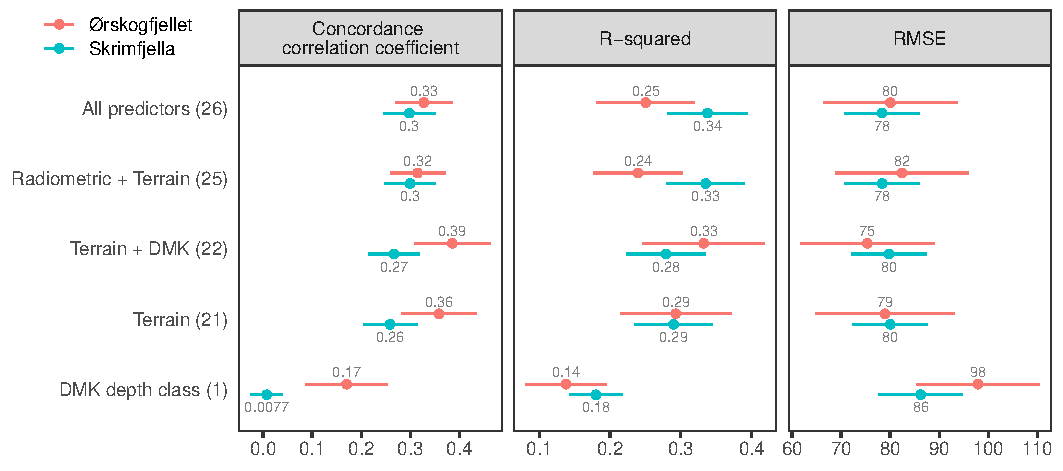
\includegraphics{figures/modelmetrics.pdf}
\caption{\label{fig:modelMetrics}Performance of peatland depth models with different predictor configurations, evaluated via spatial cross-validation. Parentheses denote the number of variables in each predictor configuration, and point estimates are shown +/- their standard error.}
\end{figure}

Although the difficulty of predicting peat depth caused prediction intervals to be wide, these uncertainty estimates were well-calibrated.
At Skrimfjella the prediction interval coverage probability was 91 \%, and at Ørskogfjellet it was 84 \% (both compared to the target value of 90 \%).
Observations outside of the prediction intervals were evenly distributed across each of the study areas.

For Skrimfjella, the best predictor configuration was \emph{all predictors}, followed closely by \emph{terrain and radiometric}.
The performance gap between the \emph{terrain and DMK} configuration and the \emph{terrain-only} configuration was similarly small.
Compared to the \emph{terrain-only} configuration, the \emph{terrain and radiometric} configuration improved concordance correlation by 0.04, R\textsuperscript{2} by 0.04, and mean absolute error by \unit{1\,cm}.
\emph{DMK class} alone -- although calibrated to measured depths -- was a very poor predictor of peat depth, with a concordance correlation coefficient of 0.008.

For Ørskogfjellet, the best predictor configuration was \emph{terrain and DMK}, followed by \emph{terrain-only}.
Adding radiometric predictors to these configurations worsened model performance, especially in terms of concordance correlation and R\textsuperscript{2}.
By itself, \emph{DMK class} produced a concordance correlation coefficient of 0.17 (compared to 0.008 at Skrimfjella), but the worst mean absolute error of any model at either site: \unit{77\,cm}.

When we tested how well models extrapolated from within to outside of mapped peatland, we found that the models produced worse mean absolute error than just assuming a constant \unit{30\,cm} depth (Fig. \ref{fig:modelMetricsExtrapolation}).
With the independent occurrence data at Skrimfjella, we found that neither the \emph{terrain-only} nor \emph{terrain and radiometric} configurations were able to discriminate between peat presence and absence (area under the curve of the receiver operating characteristic 0.44 and 0.52 respectively, where 0.5 indicates random guessing).

\begin{figure}
\centering
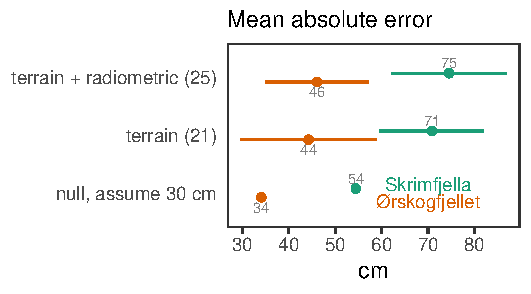
\includegraphics{figures/modelmetrics-extrapolation.pdf}
\caption{\label{fig:modelMetricsExtrapolation}Performance of models that extrapolate from training data inside of mapped peatland to test data outside of mapped peatland, evaluated via spatial cross-validation. Parentheses denote the number of variables in each model, and point estimates are shown +/- their standard error.}
\end{figure}

For the purpose of model interpretation, the \emph{all predictors} configuration for Skrimfjella was reduced from 27 variables to 11 non-collinear variables.
Similarly, the \emph{terrain and DMK} configuration for Ørskogfjellet was reduced from 23 variables to 11 non-collinear variables.
At both sites, \emph{elevation} and \emph{MRVBF} were important predictors (Fig. \ref{fig:varImp}).
At Skrimfjella these two predictors were of similar importance, while at Ørskogfjellet \emph{elevation} was more important than \emph{MRVBF}.
\emph{DMK} was also important -- the shallow class in particular -- but only at Ørskogfjellet.
Some realizations of the hydrological predictors \emph{TWI} and \emph{DTW} showed considerable importance, while others showed little -- with no consistency between sites.
For example, \emph{TWI5m}, \emph{DTW40000}, and \emph{DTW2500} rounded out the top five most important variables at Skrimfjella, while \emph{TWI20m} and \emph{TWI50m} were least important, other than \emph{DMK}.
At both sites, the most important realizations of hydrological predictors were more important than the simple terrain indices \emph{slope}, \emph{TRI}, \emph{TPI}, and \emph{roughness}.
The radiometric variable \emph{radU} showed moderate importance at Skrimfjella.

\begin{figure}
\centering
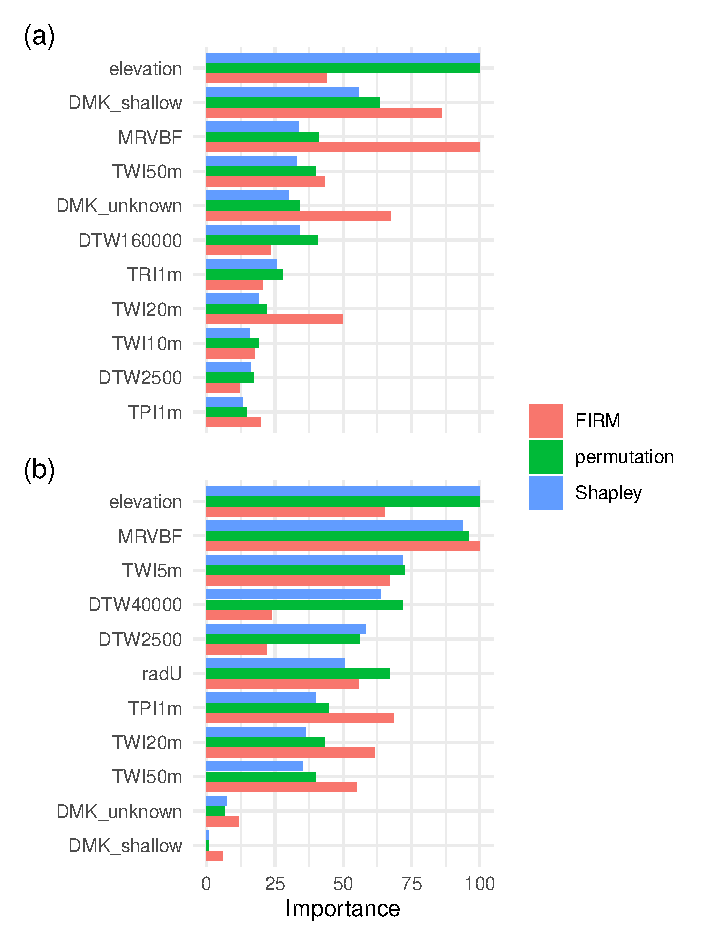
\includegraphics{figures/variable_importance.pdf}
\caption{\label{fig:varImp}Global variable importance in the best-performing models at Ørskogfjellet (a) and Skrimfjella (b), as measured by three different metrics. Variables removed due to collinearity are shown to the right of that with which they are most correlated.}
\end{figure}

Many of the the most important predictors in the best performing models showed non-monotonic effects on peat depth (Fig. \ref{fig:pdps}).
At Ørskogfjellet for example, increasing \emph{elevation} was predictive of deeper peat up to about 75 meters above sea level, after which a further increase was predictive of shallower peat.
At Skrimfjella the partial dependence on \emph{elevation} had the opposite shape, with the shallowest peats predicted at intermediate elevations, around 350 meters above sea level.
\emph{TWI50m} at Ørskogfjellet and \emph{DTW4000} and \emph{radU} at Skrimfjella were other predictors that showed considerable fluctuations in their predictive effects on peat depth.
The radiometric predictor in particular displayed an idiosyncratic effect, with a marked dip in predicted depth at intermediate values of \emph{radU}.
On the other hand, the partial effects of some important predictors were more straightforward.
The partial dependence on \emph{MRVBF} was quite similar across sites, with the deepest peats predicted in the very flattest valley bottoms.
Also, \emph{TWI5m} and \emph{DTW2500} at Skrimfjella showed monotonically positive and negative predictive effects, respectively.

Individual conditional expectation lines indicated some interactions between predictors (Fig. \ref{fig:pdps}).
For example, the magnitude of the increase in depth with \emph{elevation} that the model expected at Ørskogfjellet was different for different observations; some depth predictions increased by only \unit{40\,cm} while others increased by more than \unit{100\,cm}, over the same elevation gain.
Similarly, ICE lines of \emph{radU} at Skrimfjella were non-parallel, with some locations showing monotonically increasing peat depth predictions with uranium concentration (unlike the average effect).
Nevertheless, most ICE lines were generally parallel -- indicating that the average effects of the predictors were good representations of their overall effects.

\begin{figure}
\centering
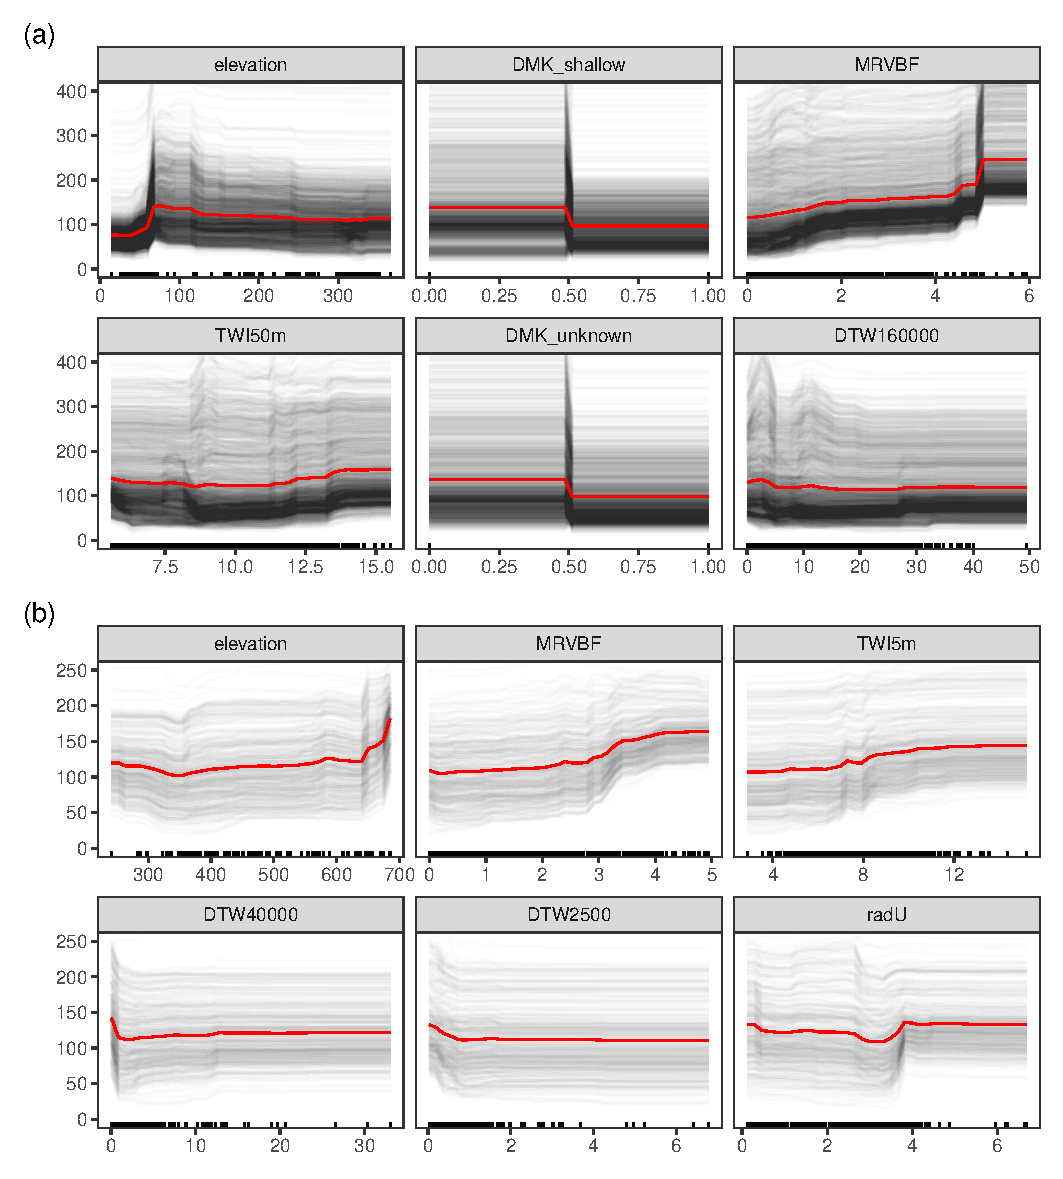
\includegraphics{figures/partial_dependence.pdf}
\caption{\label{fig:pdps}Partial dependence plots of the six most important variables in the best-performing models at Ørskogfjellet (a) and Skrimfjella (b). The average effect of the predictor on the outcome (red line) overlays the variation in the effect across observations (grey lines).}
\end{figure}

\section{Discussion}

Lorem ipsum dolor sit amet, consectetur adipiscing elit.
Sed do eiusmod tempor incididunt ut labore et dolore magna aliqua.
Ut enim ad minim veniam, quis nostrud exercitation ullamco laboris nisi ut aliquip ex ea commodo consequat.
Duis aute irure dolor in reprehenderit in voluptate velit esse cillum dolore eu fugiat nulla pariatur.
Excepteur sint occaecat cupidatat non proident,
sunt in culpa qui officia deserunt mollit anim id est laborum.

\section{Conclusions}

Nulla facilisi.
Maecenas vel nunc nec purus tincidunt congue.
Proin auctor, lectus eu pharetra malesuada,
nisi nunc bibendum nunc,
eget tincidunt nunc nisi id nunc.
Sed euismod, nunc sit amet aliquam tincidunt,
nunc nunc tincidunt nunc,
nec tincidunt nunc nunc nec nunc.
Donec auctor, nunc sit amet aliquam tincidunt,
nunc nunc tincidunt nunc,
nec tincidunt nunc nunc nec nunc.



\codedataavailability{\emph{Code and data availability.} Use this to add a statement when having data sets and software code available} %% use this section when having data sets and software code available



%%%%%%%%%%%%%%%%%%%%%%%%%%%%%%%%%%%%%%%%%%
%% optional

%%%%%%%%%%%%%%%%%%%%%%%%%%%%%%%%%%%%%%%%%%

%%%%%%%%%%%%%%%%%%%%%%%%%%%%%%%%%%%%%%%%%%
\authorcontribution{\emph{Author contributions.}
JV: Conceptualization, Investigation, Data curation, Formal analysis, Writing -- original draft.
NG: Conceptualization, Methodology, Writing - review \& editing.
MKG: Investigation, Writing - review \& editing.
KKM: Investigation, Data curation, Writing - review \& editing.
SDN: Investigation, Writing - review \& editing.
KR: Conceptualization, Investigation, Writing - review \& editing.
MS: Investigation, Data curation, Writing - review \& editing.} %% optional section

%%%%%%%%%%%%%%%%%%%%%%%%%%%%%%%%%%%%%%%%%%
\competinginterests{\emph{Competing interests.} The authors declare that they have no conflict of interest.} %% this section is mandatory even if you declare that no competing interests are present

%%%%%%%%%%%%%%%%%%%%%%%%%%%%%%%%%%%%%%%%%%
\disclaimer{\emph{Disclaimer.} The authors declare that the results, discussions, and interpretations presented in this study are solely their own. The views expressed herein do not necessarily reflect those of their respective institutions or funding agencies.} %% optional section

%%%%%%%%%%%%%%%%%%%%%%%%%%%%%%%%%%%%%%%%%%
\begin{acknowledgements}
\emph{Acknowledgements.} We thank the Norwegian Public Roads Administration for sharing data from ground-penetrating radar surveys. We also thank Vikas Baranwal from the Geological Survey of Norway for helping us access the radiometric data from Skrim. This work contains data under the following licenses: (1) Creative Commons Attribution 4.0 International, © Kartverket, (2) \emph{Norge digitalt} license, Norwegian Institute of Bioeconomy Research (NIBIO), © Geovekst, and (3) the Norwegian License for Public Data (NLOD), made available by the Geological Survey of Norway (NGU). Large language models have been used during the drafting and editing of this manuscript, with author oversight. We maintain full responsibility for the scientific output, as per the European Commission's \emph{Living guidelines on the responsible use of generative AI in research}.
\end{acknowledgements}

%% REFERENCES
%% DN: pre-configured to BibTeX for rticles

%% The reference list is compiled as follows:
%%
%% \begin{thebibliography}{}
%%
%% \bibitem[AUTHOR(YEAR)]{LABEL1}
%% REFERENCE 1
%%
%% \bibitem[AUTHOR(YEAR)]{LABEL2}
%% REFERENCE 2
%%
%% \end{thebibliography}

%% Since the Copernicus LaTeX package includes the BibTeX style file copernicus.bst,
%% authors experienced with BibTeX only have to include the following two lines:
%%
\bibliographystyle{copernicus}
\bibliography{ms.bib}
%%
%% URLs and DOIs can be entered in your BibTeX file as:
%%
%% URL = {http://www.xyz.org/~jones/idx_g.htm}
%% DOI = {10.5194/xyz}


%% LITERATURE CITATIONS
%%
%% command                        & example result
%% \citet{jones90}|               & Jones et al. (1990)
%% \citep{jones90}|               & (Jones et al., 1990)
%% \citep{jones90,jones93}|       & (Jones et al., 1990, 1993)
%% \citep[p.~32]{jones90}|        & (Jones et al., 1990, p.~32)
%% \citep[e.g.,][]{jones90}|      & (e.g., Jones et al., 1990)
%% \citep[e.g.,][p.~32]{jones90}| & (e.g., Jones et al., 1990, p.~32)
%% \citeauthor{jones90}|          & Jones et al.
%% \citeyear{jones90}|            & 1990


\end{document}
